\documentclass{beamer}

\mode<presentation> {
\usetheme{Madrid}
\usecolortheme{beaver}
%\usecolortheme{orchid}
%\usecolortheme{wolverine}

%\setbeamertemplate{footline} % To remove the footer line in all slides uncomment this line
\setbeamertemplate{footline}[page number] % To replace the footer line in all slides with a simple slide count uncomment this line

\setbeamertemplate{navigation symbols}{} % To remove the navigation symbols from the bottom of all slides uncomment this line
}

\usepackage{graphicx}
\usepackage{booktabs}

%\usepackage {xcolor}
\definecolor {processblue}{cmyk}{0.96,0,0,0}
\definecolor {upmBlue}{rgb}{0.2, 0.6745, 1}

% -------------
% BEGIN - TITLE
% -------------

\title[Short title]{Proyecto de Inteligencia Artificial}

\author{Rubén Aguado Cosano - z170284 \\ Younes Aguado Cosano - z170284 \\ Paula Pousa Cosano - z170284 \\ Jorge Sol Gonzalez - z170212}

\institute[ETSIINF UPM] 
{
  \textcolor{upmBlue}{Universidad Politecnica de Madrid}\\
\medskip
}
\date{\today}

\begin{document}

\begin{frame}
\titlepage
\end{frame}

\begin{frame}
\frametitle{Indice}
\tableofcontents
\end{frame}

% -----------
% END - TITLE
% -----------

%---------------------
%	BEGIN - PRESENTATION
%---------------------

\section{Magnitud y Coordenadas}
\begin{frame}{Magnitud del problema y coordenadas de las estaciones.}
    \begin{itemize}
        \item La magnitud de medida elegida se ha realizado en metros.
        \item Para las lineas rectas sobre el plano se utilizaron las coordenadas de las estaciones cogidas de google maps.
        \vspace{0.5cm}
        \begin{figure}[H]
         \centering
         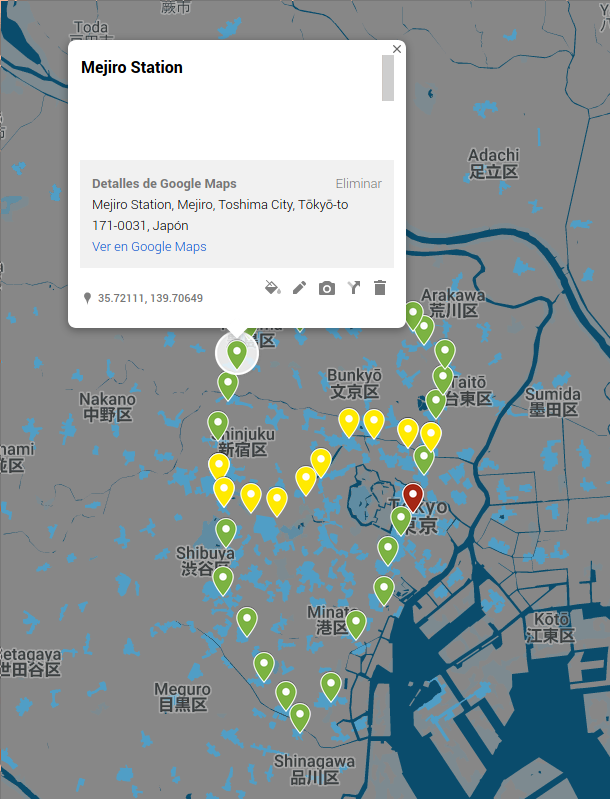
\includegraphics[scale=0.20]{"../pics/ejemploCoordenadas.png"}
        \end{figure}
    \end{itemize}
\end{frame}

\begin{frame}{Magnitud del problema y coordenadas de las estaciones.}
  \begin{itemize}
    \item Una vez recogidas las coordenadas de todas las estaciones.
    \item Aplicamos la formula de Haversine para calcular las distancias rectas.
  \end{itemize}
  \begin{figure}[H]
    \centering
    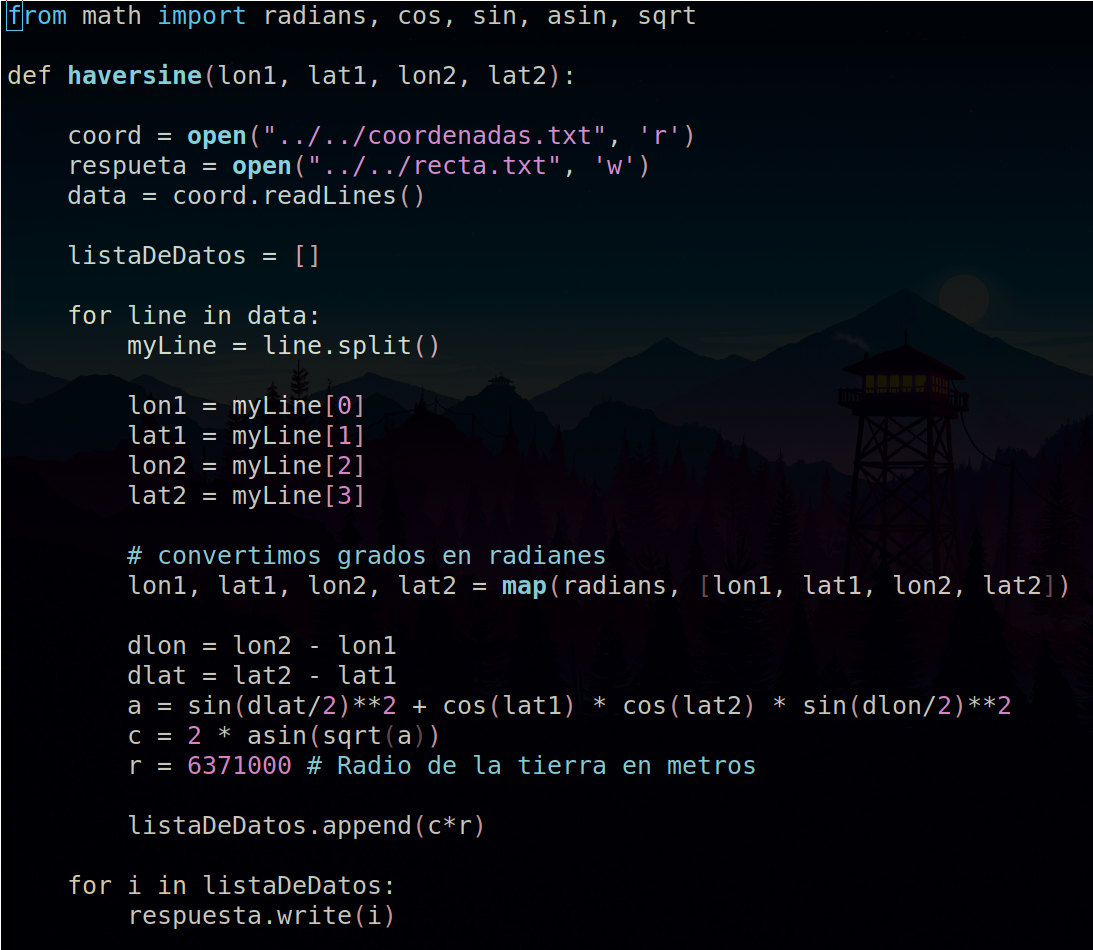
\includegraphics[scale=0.20]{"../pics/haversine.png"}
  \end{figure}
\end{frame}

\section{Distancias Reales}
\begin{frame}{Calculo de las distancias reales y recogida de tiempos.}
  \begin{itemize}
    \item La recogida de las distancias reales se realizó a mano con ayuda de la página web \textcolor{red}{HyperDia}
    \vspace{0.5cm}
    \begin{figure}[H]
      \centering
      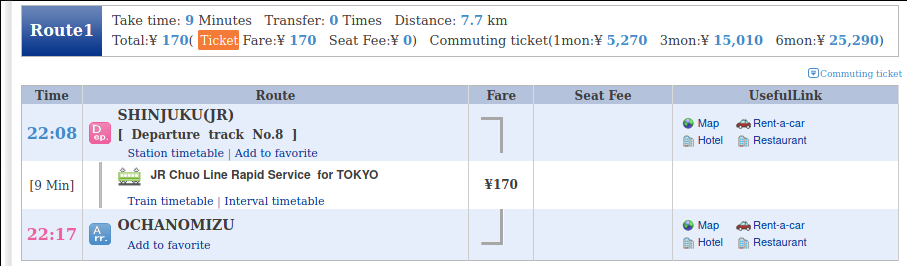
\includegraphics[scale=0.30]{"../pics/hyperDia.png"}
    \end{figure}
  \end{itemize}
\end{frame}

\section{Base de Datos}
\begin{frame}{Almacenamiento de los datos en una Base de Datos sqlite3}
    \begin{itemize}
        \item Para recuperar la información, hemos hecho uso de una BDD sqlite3.
        \vspace{0.2cm}
        \begin{figure}[H]
          \centering
          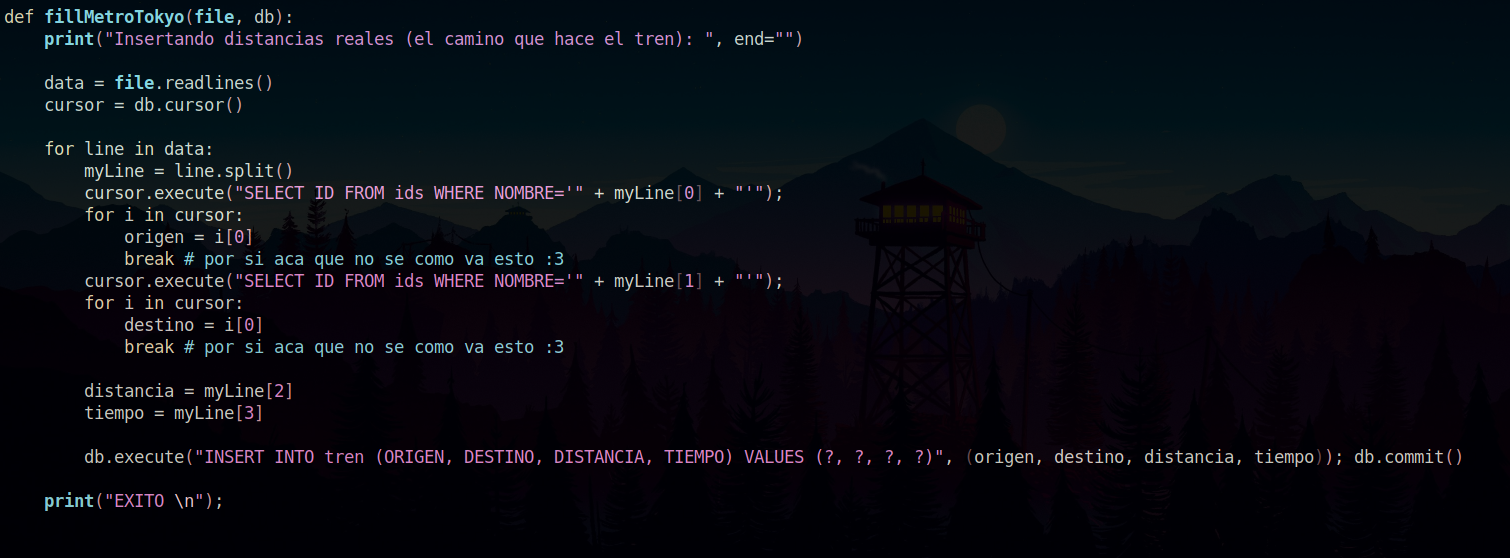
\includegraphics[scale=0.20]{"../pics/bddCodigo.png"}
        \end{figure}
    \end{itemize}
\end{frame}
\begin{frame}{Almacenamiento de los datos en una Base de Datos sqlite3}
  \begin{figure}[H]
    \centering
    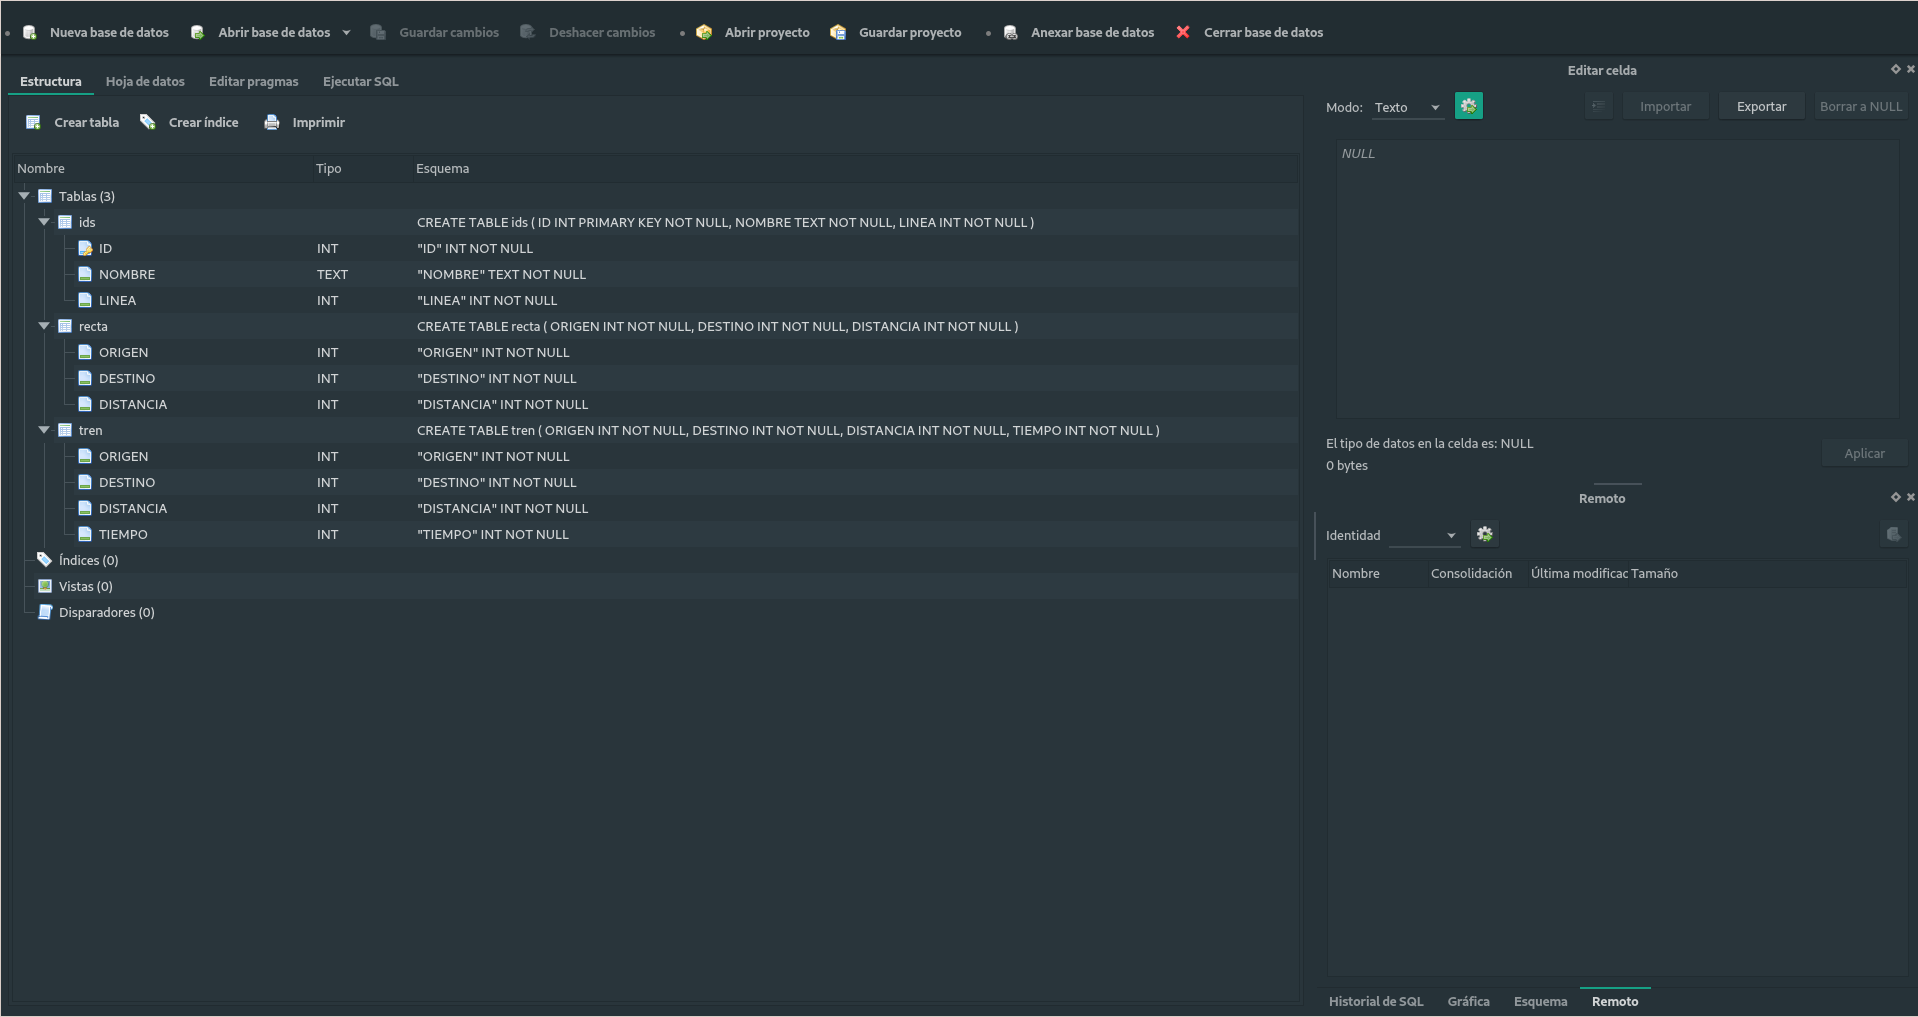
\includegraphics[scale=0.17]{"../pics/bdd.png"}
  \end{figure}
\end{frame}

\begin{frame}
  \Huge{\centerline{Gracias :)}}
\end{frame}

%---------------------
%	END - PRESENTATION
%---------------------

\end{document}
